% Subgame perfection: the Traitors, then backwards induction on the centipede.
% Shared preamble for the write-on class slides.
%
% Every deck is designed to be projected and annotated live on a tablet:
% whatever takes time to draw is pre-drawn, and whatever the class produces is
% left blank. Compile a deck with `pdflatex main.tex` from its own directory,
% or run `make` in decks/ to build them all.
\documentclass[10pt]{article}

\usepackage[papersize={25.6cm,14.4cm}, margin=1.1cm, bottom=1.5cm,
            footskip=0.75cm]{geometry}
\usepackage[T1]{fontenc}
\usepackage[default]{sourcesanspro}
\usepackage{newtxsf}
\usepackage{tikz}
\usepackage{amsmath}
\usepackage{parskip}
\usepackage{fancyhdr}
\usetikzlibrary{arrows.meta, positioning, calc}

\setlength{\parindent}{0pt}

% Catppuccin Latte, the palette the course site uses in its light theme, so a
% deck on the projector looks like the pages the students read.
\definecolor{inkbg}{HTML}{EFF1F5}      % base
\definecolor{inksurface}{HTML}{E6E9EF} % mantle
\definecolor{inkfaint}{HTML}{CCD0DA}   % surface2, for rules and empty boxes
\definecolor{inktext}{HTML}{4C4F69}    % text
\definecolor{inkgrey}{HTML}{8C8FA1}    % overlay1, for anything secondary
\definecolor{inkblue}{HTML}{7287FD}    % lavender, the primary accent
\definecolor{inkteal}{HTML}{179299}    % teal
\definecolor{inkred}{HTML}{FE640B}     % peach, for whatever wants attention
\definecolor{inkmauve}{HTML}{8839EF}   % mauve

\pagecolor{inkbg}
\color{inktext}

% A box to write a number into. White against the tinted page, so it reads as
% somewhere to write rather than as part of the printed material.
\newcommand{\blank}[1][1.6]{%
  \tikz[baseline=(current bounding box.base)]{%
    \draw[inkfaint, line width=0.7pt, rounded corners=2pt, fill=white]
      (0,-0.18) rectangle (#1,0.62);}}

% A ruled area to work in. Faint dots keep handwriting level on a tablet.
\newcommand{\workspace}[2]{%
  \begin{tikzpicture}
    \draw[inkfaint, line width=0.7pt, rounded corners=3pt, fill=white]
      (0,0) rectangle (#1,#2);
    \foreach \gx in {0.5,1.0,...,#1}{%
      \foreach \gy in {0.5,1.0,...,#2}{%
        \fill[inkfaint] (\gx,\gy) circle (0.5pt);}}
  \end{tikzpicture}}

% A panel for material that is printed rather than written on.
\newcommand{\panel}[2]{%
  \begin{tikzpicture}
    \draw[inkfaint, line width=0.7pt, rounded corners=3pt, fill=inksurface]
      (0,0) rectangle (#1,#2);
  \end{tikzpicture}}

% An empty payoff grid. #1 is the list of action names, #2 is drawn afterwards
% so a page can add its own marks.
\newcommand{\payoffgrid}[2]{%
  \begin{tikzpicture}[scale=1.0, every node/.style={transform shape}]
    \foreach \name [count=\j from 0] in {#1}{%
      \node[font=\bfseries, text=inkblue] at (\j*2.7+1.35,0.55) {\name};
      \node[font=\bfseries, text=inkblue] at (-1.15,-\j*2-1) {\name};
      \foreach \k [count=\i from 0] in {#1}{%
        \draw[inkfaint, line width=0.7pt, fill=white]
          (\j*2.7,-\i*2) rectangle (\j*2.7+2.7,-\i*2-2);}}
    #2
  \end{tikzpicture}}

% The five actions on a pentagon. Each action beats the one next to it and the
% one across from it, so the two winning cycles are drawn as separate panels:
% ten labelled arrows on one diagram is a tangle nobody can read from the back
% of the room.
\newcommand{\rpslscycle}[3]{%
  \begin{tikzpicture}[scale=1.0, every node/.style={transform shape},
      >={Stealth[length=2.6mm]},
      action/.style={circle, draw=inkfaint, line width=1pt, fill=white,
                     text=inktext, minimum size=1.7cm, inner sep=1pt,
                     font=\small\bfseries},
      beats/.style={->, line width=1.2pt, shorten >=3pt, shorten <=3pt,
                    draw=#1},
      word/.style={font=\scriptsize, fill=inkbg, inner sep=1.6pt, text=#1,
                   sloped, pos=#2}]
    \foreach \name/\angle in {Rock/90, Lizard/18, Spock/-54,
                              Scissors/-126, Paper/162}{%
      \node[action] (\name) at (\angle:3.1) {\name};}
    \foreach \winner/\loser/\said in {#3}{%
      \draw[beats] (\winner) -- node[word] {\said} (\loser);}
  \end{tikzpicture}}

% Running header: the deck name on the left, the page's own step on the right.
% Each deck sets its name once with \deckname.
\newcommand{\deck}{}
\newcommand{\deckname}[1]{\renewcommand{\deck}{#1}}
\newcommand{\slidehead}[1]{%
  {\small\color{inkgrey}%
   \tikz[baseline=-0.5ex]{\fill[inkblue, rounded corners=1pt]
     (0,0) rectangle (0.22,0.22);}\;\deck
   \hfill \color{inkblue}\bfseries #1}\par
  {\color{inkblue}\rule{\linewidth}{1pt}}\par\vspace{0.35em}}

\pagestyle{fancy}
\fancyhf{}
\renewcommand{\headrulewidth}{0pt}
\fancyfoot[R]{\small\color{inkgrey}\thepage}

% Deck title pages, which carry no header and no page number.
\newcommand{\titleslide}[3]{%
  \thispagestyle{empty}%
  \begin{center}
    \vspace*{\fill}
    {\Huge\bfseries\color{inkblue} #1}\\[0.7em]
    {\LARGE\color{inkgrey} #2}\\[2.4em]
    #3
    \vspace*{\fill}
  \end{center}}

% One step of the plan on a title page.
\newcommand{\stepbox}[3]{%
  \node[draw=inkblue, line width=0.9pt, rounded corners=4pt, fill=white,
        minimum width=6cm, minimum height=1.7cm, align=center,
        text=inktext] (#1) at (#2,0) {#3};}


\deckname{Subgame perfection}

\begin{document}

\titleslide{Subgame perfection}{A threat that stops being worth carrying out}{%
    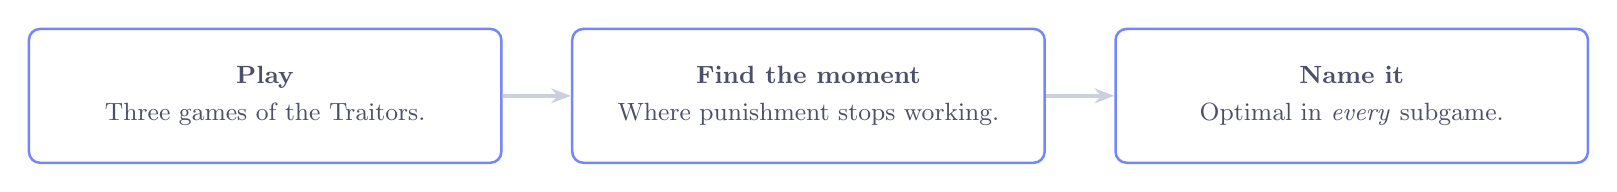
\begin{tikzpicture}[font=\small]
      \stepbox{s0}{0.0}{\textbf{Play}\\[0.25em] Three games of the Traitors.}
      \stepbox{s1}{6.9}{\textbf{Find the moment}\\[0.25em]
                          Where punishment stops working.}
      \stepbox{s2}{13.8}{\textbf{Name it}\\[0.25em] Optimal in \emph{every} subgame.}
      \draw[-{Stealth[length=2.5mm]}, inkfaint, line width=1.2pt] (s0) -- (s1);
      \draw[-{Stealth[length=2.5mm]}, inkfaint, line width=1.2pt] (s1) -- (s2);
    \end{tikzpicture}

    \vspace{2.4em}

    {\large Players: \blank[2] \hspace{1.4cm} Traitors: \blank[2]
   \hspace{1.4cm} Who won? \blank[3]}}

\newpage
\slidehead{Every round costs two players}

\vspace{0.7cm}

\begin{center}
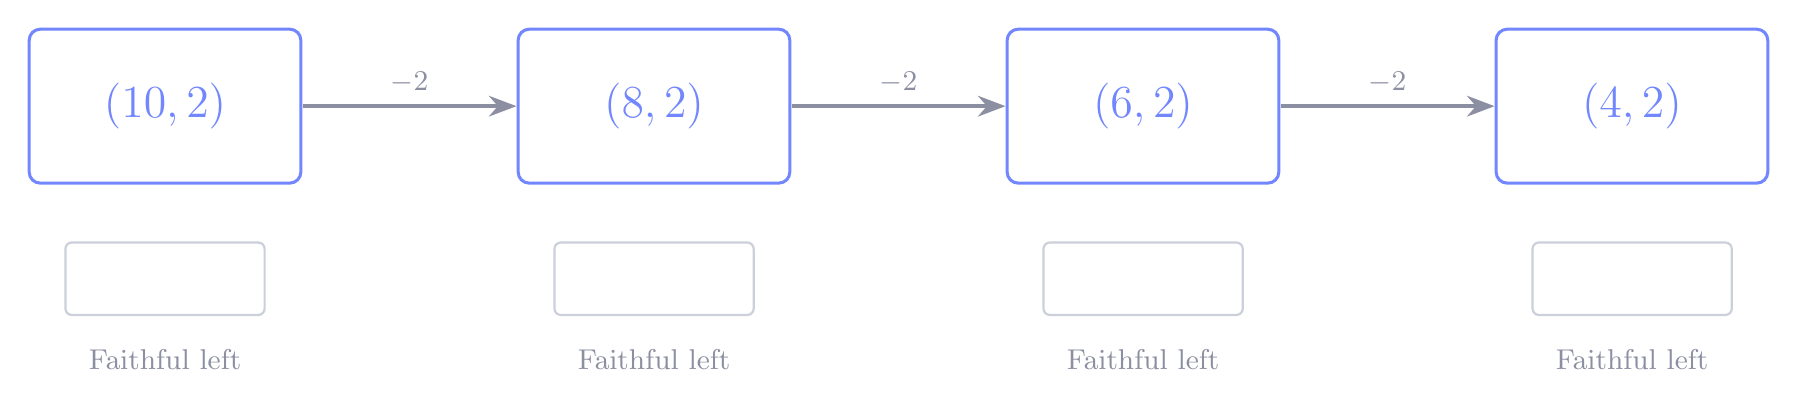
\begin{tikzpicture}[font=\large, scale=1.15,
    every node/.style={transform shape},
    state/.style={draw=inkblue, line width=1.1pt, rounded corners=4pt,
                  fill=white, minimum width=3cm, minimum height=1.7cm,
                  text=inkblue,
                  font=\Large\bfseries}]
  \foreach \lab [count=\i from 0] in {{$(10,2)$}, {$(8,2)$}, {$(6,2)$}, {$(4,2)$}}{%
    \node[state] (s\i) at (\i*5.4,0) {\lab};
    \node[below=0.5cm of s\i] {\blank[2.2]};
    \node[below=1.7cm of s\i, font=\small, text=inkgrey]
      {Faithful left};}
  \foreach \i in {0,1,2}{%
    \pgfmathtruncatemacro{\j}{\i+1}
    \draw[-{Stealth[length=3.5mm]}, inkgrey, line width=1.3pt]
      (s\i) -- node[above, font=\small, text=inkgrey] {$-2$} (s\j);}
\end{tikzpicture}

\vspace{0.5cm}

{\small\color{inkgrey} Each round loses one player to the day vote and one to
the night murder.}
\end{center}

\vspace{1.1cm}

{\large The Traitors win the moment \(2m \ge n\), which first happens at
\blank[2.4]. Reaching it takes \blank[1.6] rounds.}

\newpage
\slidehead{Vote-Left: everyone votes to their left}

\vspace{0.7cm}

\begin{minipage}[t]{0.47\linewidth}
\raggedright
{\large\bfseries It costs the Faithful nothing.}

\vspace{0.5em}

{\large Under full compliance each player receives exactly \blank[1.4] vote,
so the chance of being banished is \blank[1.6], the same as voting at
random.}

\vspace{0.8em}

\workspace{10.6}{3.6}
\end{minipage}
\hfill
\begin{minipage}[t]{0.47\linewidth}
\raggedright
{\large\bfseries It makes deviation visible.}

\vspace{0.5em}

{\large If a Traitor concentrates their vote, somebody gets \blank[1.4] votes
and somebody gets \blank[1.4]. Everyone can see who broke the rule.}

\vspace{0.8em}

\workspace{10.6}{3.6}
\end{minipage}

\vspace{0.9cm}

{\large So the punishment is: a player seen to deviate is
\underline{\hspace{4.5cm}}.}

\newpage
\slidehead{Where the threat stops being credible}

\vspace{0.9cm}

{\large At \((6,2)\) a Traitor who deviates is still detected. But after the
night murder, are there enough Faithful left to banish them? \blank[2.4]}

\vspace{1.1cm}

{\large So the threat bites exactly while}

\vspace{0.6cm}

\begin{center}
{\Huge \(n \;\)\blank[1.6]\( \; 2m + 2\)}
\end{center}

\vspace{1.1cm}

{\large Below that line the Traitors should stop hiding and collude in the open.
That is their best response \emph{in that subgame}, whether or not any game we
played actually reached it.}

\newpage
\slidehead{The centipede game}

\vspace{0.4cm}

\begin{center}
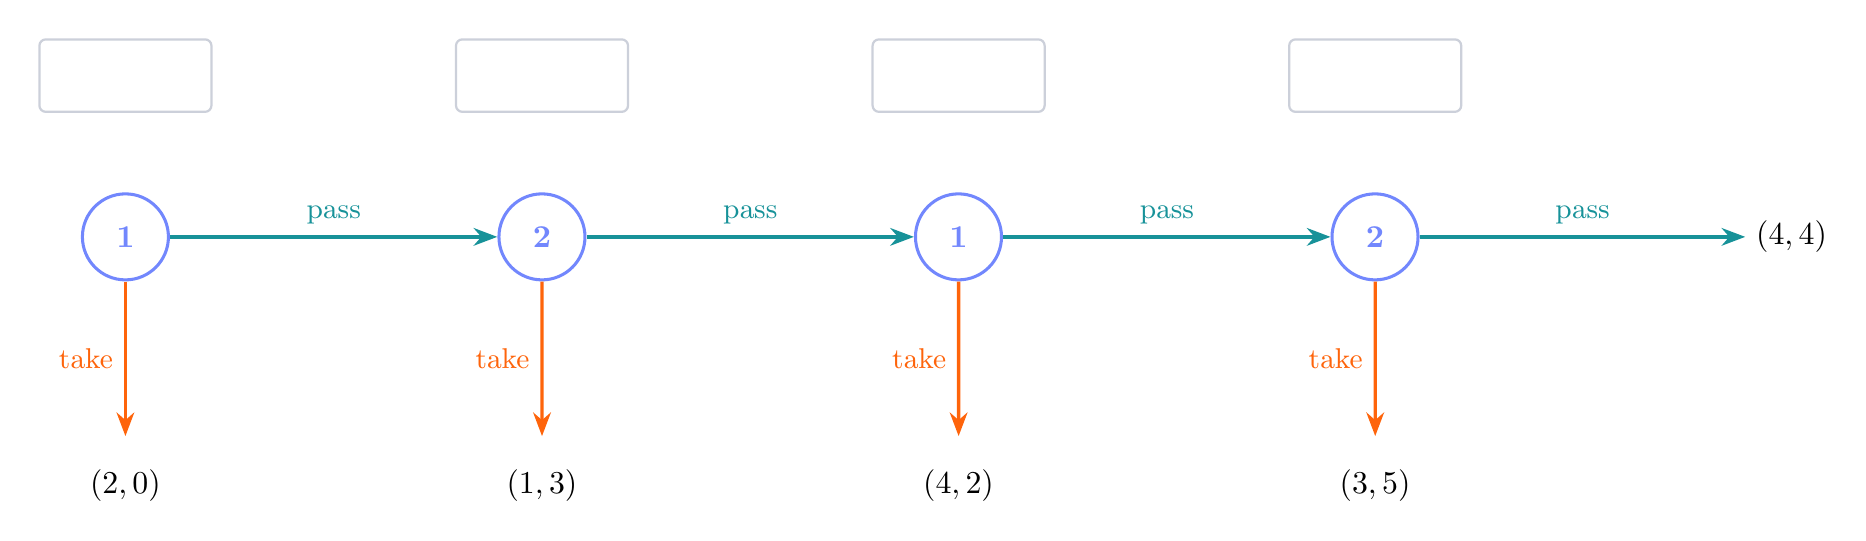
\begin{tikzpicture}[font=\small, scale=1.15,
    every node/.style={transform shape},
    dec/.style={circle, draw=inkblue, line width=1.1pt, fill=white,
                text=inkblue, minimum size=0.95cm, font=\bfseries,
                inner sep=0pt},
    leaf/.style={font=\normalsize}]
  \foreach \who [count=\i from 0] in {1, 2, 1, 2}{%
    \node[dec] (n\i) at (\i*4.6,0) {\who};
    \node[above=0.75cm of n\i] {\blank[1.9]};}
  \node[leaf] (end) at (18.4,0) {$(4,4)$};
  \foreach \pay [count=\i from 0] in {{$(2,0)$}, {$(1,3)$}, {$(4,2)$}, {$(3,5)$}}{%
    \draw[-{Stealth[length=3mm]}, inkred, line width=1.2pt]
      (n\i) -- node[left, font=\small, text=inkred] {take} ++(0,-2.2);
    \node[leaf] at (\i*4.6,-2.75) {\pay};}
  \foreach \i in {0,1,2}{%
    \pgfmathtruncatemacro{\j}{\i+1}
    \draw[-{Stealth[length=3mm]}, inkteal, line width=1.2pt]
      (n\i) -- node[above, font=\small, text=inkteal] {pass} (n\j);}
  \draw[-{Stealth[length=3mm]}, inkteal, line width=1.2pt]
    (n3) -- node[above, font=\small, text=inkteal] {pass} (end);
\end{tikzpicture}
\end{center}

\vspace{0.5cm}

{\large\color{inkgrey} Work right to left. Write the value of each node in the
box above it.}

\newpage
\slidehead{Nash, but not subgame perfect}

\vspace{0.5cm}

{\large Backwards induction gives: player 1 \blank[2.4], player 2
\blank[2.4], with payoffs \blank[2.4].}

\vspace{0.9cm}

{\large Now take a different plan. Player 1 takes at both of their nodes.
Player 2 takes at their first node, but \emph{passes} at their last.}

\vspace{0.8cm}

\hspace{1cm}
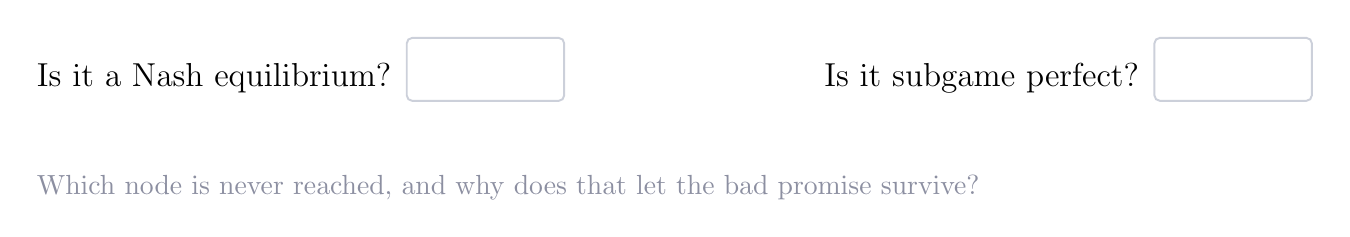
\begin{tikzpicture}[font=\large]
  \node[anchor=west] at (0,0) {Is it a Nash equilibrium? \blank[2]};
  \node[anchor=west] at (10,0) {Is it subgame perfect? \blank[2]};
  \node[anchor=west, text=inkgrey, font=\normalsize] at (0,-1.5)
    {Which node is never reached, and why does that let the bad promise
     survive?};
\end{tikzpicture}

\vspace{0.5cm}

\begin{center}
\workspace{22.6}{2.6}
\end{center}

\newpage
\slidehead{Back to the Traitors, when nobody is sure}

\vspace{0.5cm}

{\large The Traitor complies or deviates; the Faithful then banish the suspect
or carry on. The suspect is really the Traitor with probability \(q\).}

\vspace{0.5cm}

\begin{minipage}[c]{0.44\linewidth}
{\large
comply \hfill $(1, 2)$\\[1.0em]
deviate, then carry on \hfill $(3, 0)$\\[1.0em]
deviate, then banish \hfill $(3 - 8q,\; 8q - 5)$}
\end{minipage}
\hfill
\begin{minipage}[c]{0.52\linewidth}
{\small\color{inkgrey} Draw the tree:}\\[0.3em]
\workspace{12}{5.4}
\end{minipage}

\newpage
\slidehead{How sure do the Faithful have to be?}

\vspace{0.8cm}

\hspace{0.8cm}
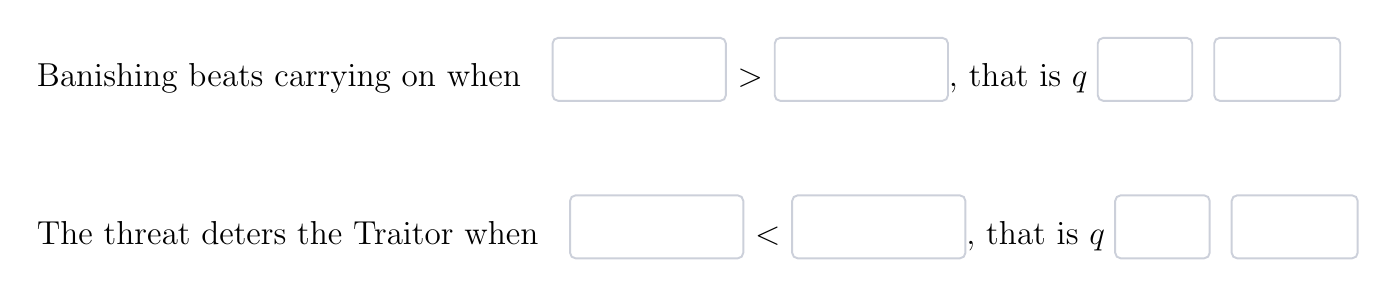
\begin{tikzpicture}[font=\large]
  \node[anchor=west] at (0,0)
    {Banishing beats carrying on when \; \blank[2.2] \(>\) \blank[2.2],
     that is \(q \;\)\blank[1.2]\( \;\) \blank[1.6]};
  \node[anchor=west] at (0,-2)
    {The threat deters the Traitor when \; \blank[2.2] \(<\) \blank[2.2],
     that is \(q \;\)\blank[1.2]\( \;\) \blank[1.6]};
\end{tikzpicture}

\vspace{1.3cm}

{\large So (comply, banish) is a Nash equilibrium that is \emph{not} subgame
perfect exactly when \(q\) lies in \blank[4].}

\vspace{0.8cm}

\begin{center}
\workspace{22.6}{2.8}
\end{center}

\newpage
\slidehead{The same thing, as an exam answer}

\vspace{0.5cm}

{\large What we just did in the room is \textbf{Question 1} on the Subgame
Perfection page.}

\vspace{0.9cm}

\hspace{0.6cm}
\begin{minipage}{0.92\linewidth}
{\large
\begin{tabbing}
\hspace{1.2cm} \= \hspace{17cm} \= \kill
\textbf{(a)} \> Draw the extensive form. \> [3]\\[0.55em]
\textbf{(b)} \> Backward induction: the subgame perfect equilibrium and its
  payoffs. \> [5]\\[0.55em]
\textbf{(c)} \> Show (comply, banish) is a Nash equilibrium. \> [5]\\[0.55em]
\textbf{(d)} \> Explain why it is not subgame perfect, and how that mirrors the
  class game. \> [6]\\[0.55em]
\textbf{(e)} \> For general \(q\), find where the threat deters and where it is
  credible. \> [4]
\end{tabbing}}
\end{minipage}

\vspace{1.2cm}

\begin{center}
{\large\color{inkgrey} vknight.org/gt/topics/subgame-perfection.html}
\end{center}

\end{document}
